\documentclass{article}
\usepackage{fullpage,graphicx,amssymb}

\def\bbD{\mathbb{D}}
\def\bbR{\mathbb{R}}
\def\arccosh{\mathrm{arccosh}}

\title{Klein distance as a Hilbert log cross-ratio distance}

\author{Frank Nielsen}
\date{2023}

\begin{document}
\maketitle

Let $\bbD$ be the unit open ball of $\bbR^d$.
Consider the Hilbert log cross-ratio distance on $(\bbD\in\bbR^d,\|\cdot\|_2)$:
\begin{equation}\label{eq:H}
\rho_H(p,q)=\frac{1}{2}\log \frac{\|p-a\|\, \|q-b\|}{\|p-b\| \, \|q-a\| },
\end{equation}
where $a,p,q,b$ are colinear, i.e., $a$ and $b$ are the two intersection points of line $(pq)$ with the boundary $\partial\bbD$ of the unit ball (Figure~\ref{fig:kg}).

To calculate $a$ and $b$, we first write the equation $ax+by+c=0$ of the line passing through $p$ and $q$:
$$
\underbrace{(p_y-q_y)}_{a}x+\underbrace{(q_x-p_x)}_{b}y+\underbrace{p_y(p_x-q_x)+p_x(q_y-p_y)}_{c}=0.
$$

Then we solve a quadratic equation induced by the system:
$$
\left\{\begin{array}{lll}
x^2+y^2 -1 &=& 0,\\
ax+by+c &=& 0.
\end{array}
\right.
$$
We write $y=\frac{-c-ax}{b}$ and expand this term in $x^2+y^2 -1=0$ to get the quadratic equation.

We have $\Delta=B^2-4AC$ with $A=1+\left(\frac{a}{b}\right)^2$, $B=\frac{2ac}{b^2}$, and $C=-1+\left(\frac{c}{b}\right)^2$:
$$
x_1=\frac{-B-\sqrt{\Delta}}{2A}, \quad x_2=\frac{-B+\sqrt{\Delta}}{2A}.
$$

We find that the Hilbert distance amounts
$$
\rho_K(p,q)=\arccosh\left( \frac{1-p\cdot q}{\sqrt{(1-p\cdot p)\, (1-q\cdot q)}}\right),
$$
where $x\cdot y$ is the Euclidean inner product and
$$
\arccosh(x)=\log(x+\sqrt{x^2-1}).
$$

Distance $\rho_K(p,q)$ is the Klein distance, the hyperbolic distance in the Klein model of hyperbolic geometry 
 

\begin{figure}%
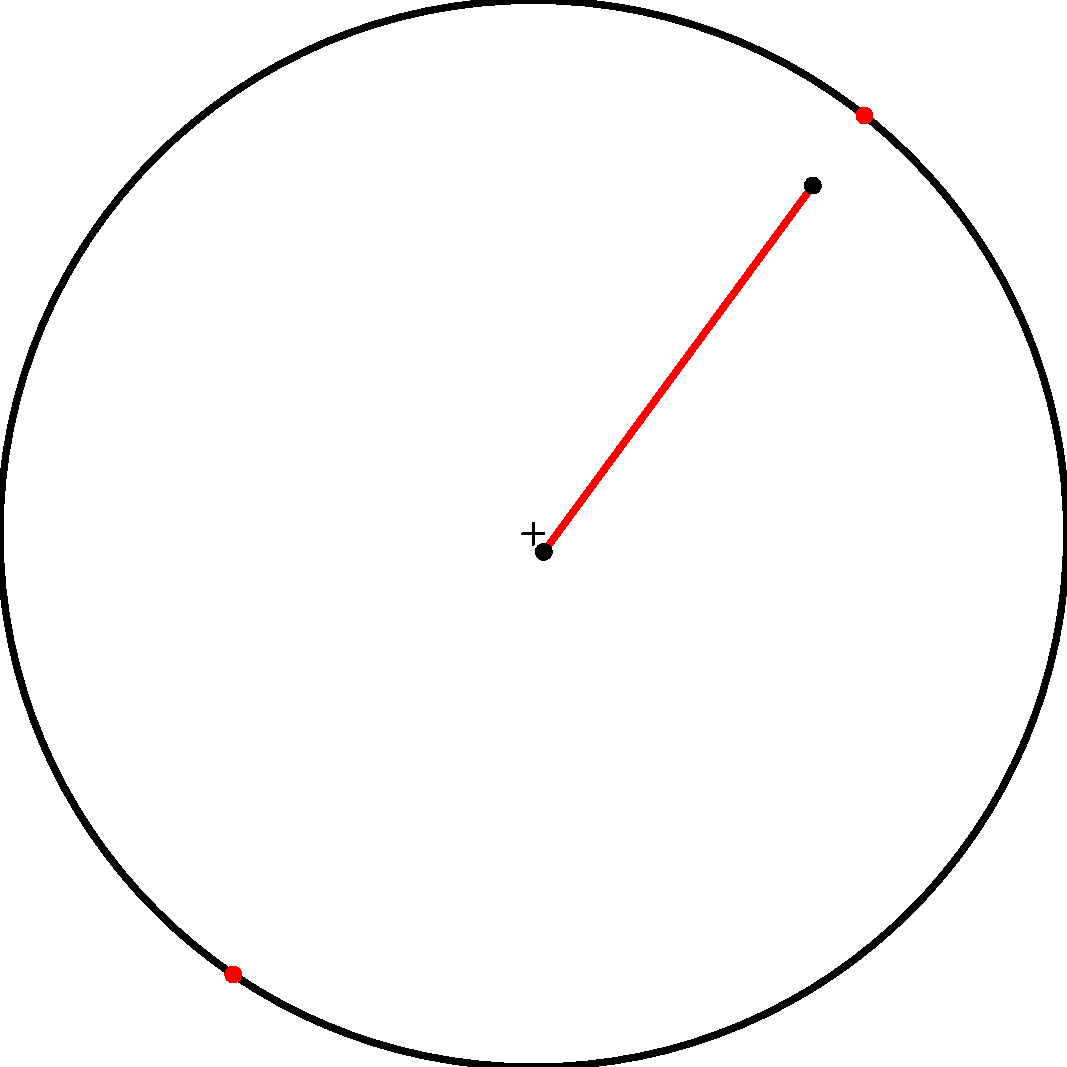
\includegraphics[width=\columnwidth]{Fig-KleinGeodesic.pdf}%
\caption{Klein geodesics are straight line segments. Klein distance is Hilbert distance induced by the open unit ball domain $\bbD$.}%
\label{fig:kg}%
\end{figure}
	

\end{document}